\chapter{Konwolucyjne sieci neuronowe}
Konwolucyjne sieci neuronowe (ang. Convolutional Neural Networks)

funkcja obrazowa;
splot;
filtr;
jądro;
warstwy konwolucyjne;
wartwy aktywacji neuronów;
warstwy FC;
Dropout;
Normalizacja;

\section{Zarys historyczny}
\section{Problem nadmiernego dopasowania}
\label{sec-overffiting}
-dropout
Kolejnym zabiegiem wykorzystywanym tym razem w celu polepszenia generalizacji klasyfikacji zbioru danych było użycie techniki dropout [Dropout].

Combining the predictions of many different models is a very successful way to reduce test errors
[1, 3], but it appears to be too expensive for big neural networks that already take several days
to train. There is, however, a very efficient version of model combination that only costs about a
factor of two during training. The recently-introduced technique, called “dropout” [10], consists
of setting to zero the output of each hidden neuron with probability 0.5. The neurons which are
“dropped out” in this way do not contribute to the forward pass and do not participate in backpropagation.
So every time an input is presented, the neural network samples a different architecture,
but all these architectures share weights. This technique reduces complex co-adaptations of neurons,
since a neuron cannot rely on the presence of particular other neurons. It is, therefore, forced to
learn more robust features that are useful in conjunction with many different random subsets of the
other neurons. At test time, we use all the neurons but multiply their outputs by 0.5, which is a
reasonable approximation to taking the geometric mean of the predictive distributions produced by
the exponentially-many dropout networks.
We use dropout in the first two fully-connected layers of Figure 2. Without dropout, our network exhibits
substantial overfitting. Dropout roughly doubles the number of iterations required to converge.

--data augmentation


-5 fold
\section{Problem redukcji wymiarowości}

\section{Przykłady współczesnych topologii}
\subsection{AlexNet}
\label{AlexNet}
Sieć AlexNet, której nazwa pochodzi od imienia głównego twórcy tej architektury Alexa Krizhevsky, zawiera blisko 60 milionów parametrów i 650 tysięcy neuronów. Architekturę zaprezentowano na Rys. \ref{AlexNetTopology}
\begin{figure}[h!]
	\centering
	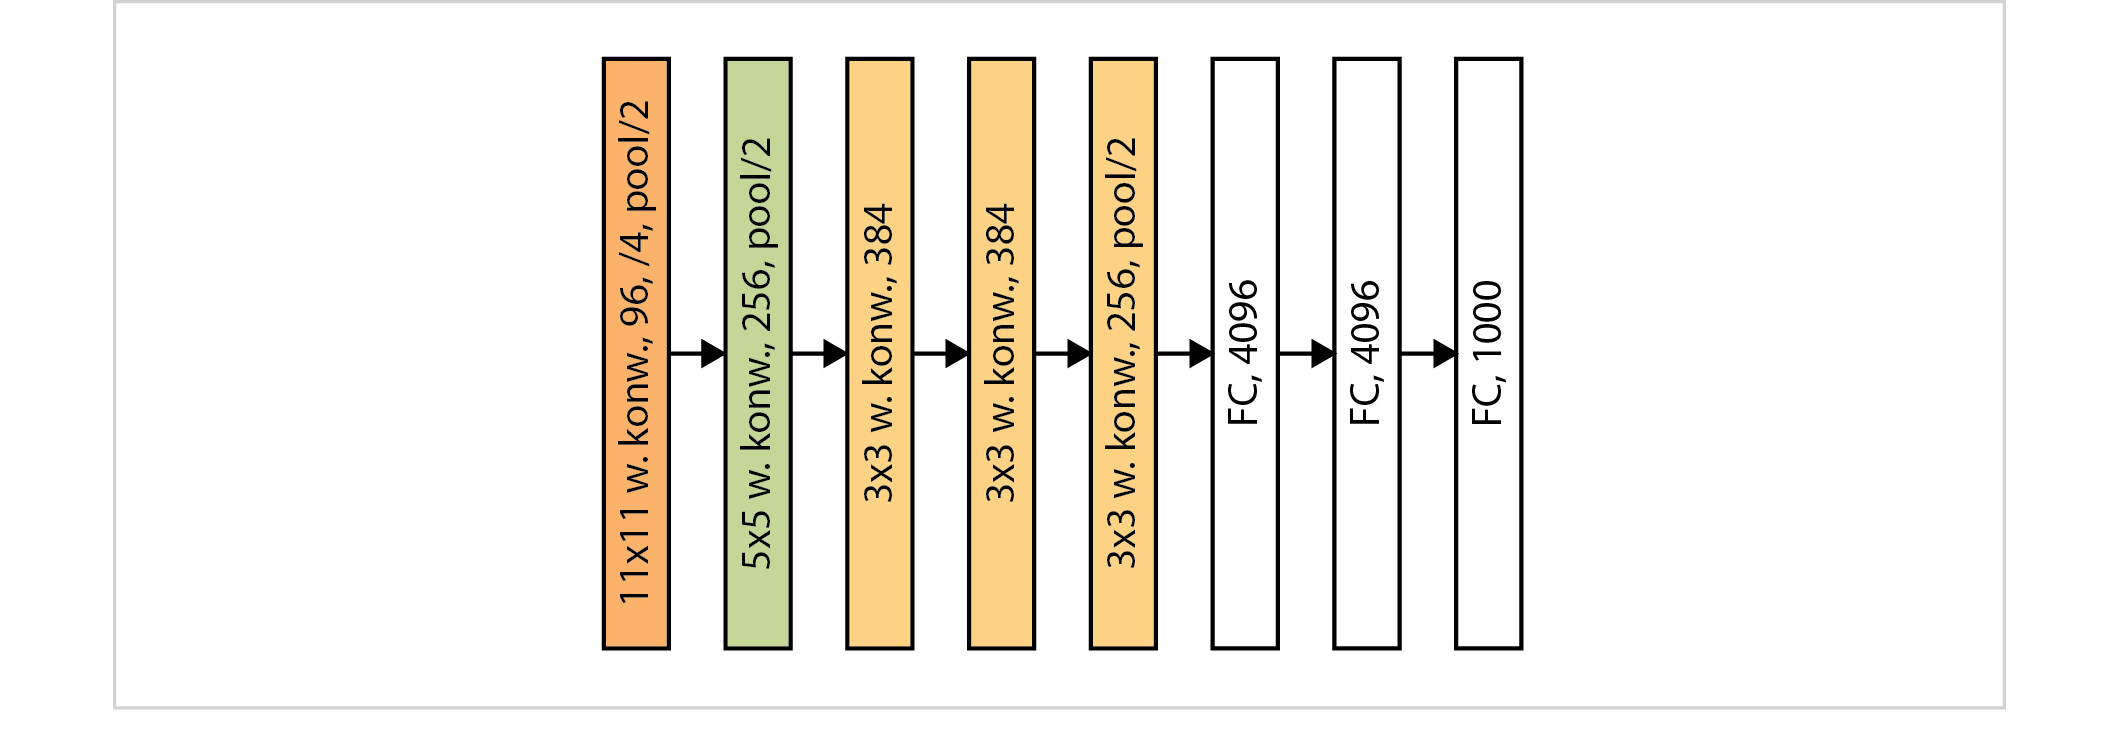
\includegraphics[width=0.55\textwidth]{figures/AlexNet.png}
	\caption{Topologia architektury AlexNet.}
	\label{AlexNetTopology}
\end{figure}

W skład topologii wchodzi pięć warstw konwolucyjnych i trzy typu fully-connected. Po pierwszej, drugiej i piątej warstwie konwolucyjnej występują operacje typu max-pool z jądrem o wymiarach 2$\times$2 \footnote{autorzy pracy podają też przykłady użycia jąder o wymiarze 2$\times$3, które nakładają się w przestrzeni funkcji obrazowej}. 

Pierwsza warstwa konwolucyjna przyjmuje na wejściu dane o wymiarze 227$\times$227$\times$3, na których wykonywana jest operacja splotu z 96 filtrami z jądrem splotu o wymiarach 11$\times$11$\times$3 i krokiem 4. W rezultacie (uwzględniając również operację max-pool) objętość wynikowa przekazywana do kolejnej warstwy ma wymiar 27$\times$27$\times$96. W drugiej warstwie konwolucyjnej wykonywana jest operacja splotu z 256 filtrami z jądrem o wymiarach 5$\times$5$\times$96. Wymiar objętości wynikowej zostaje ponownie zredukowany poprzez operacje max-pool do 13$\times$13$\times$256. Kolejne 3 warstwy konwolucyjne są połączone bezpośrednio ze sobą. Trzecia warstwa zawieraja 384 filtry o wymiarze 3$\times$3$\times$256, w skład czwartej wchodzą 384 filtry o wymiarze 3$\times$3$\times$384, a w piątej znajdują się 256 filtry ponownie o wymiarze 3$\times$3$\times$384. Końcowe dwie warstwy typu FC zawierają po 4096 neuronów, a ostatnia zawiera tyle neuronów ile klas występuje w ostatecznym podziale - w oryginalnej pracy było to 1000 [AlexNet].

W celu lepszego zrozumienia przetwarzania sygnału wejściowego przez sieć poniżej przedstawiono przykład algorytmu wykorzystywanego dla pierwszej warstwy konwolucyjnej opisywanej topologii: 
\begin{enumerate}
\item Z danych wejściowych o wymiarze [227$\times$227$\times$3] wybierany jest co czwarty blok (zarówno wzdłuż wysokości jak i szerokości) o wymiarach [11$\times$11$\times$3]. Punkty krawędziowe, które stanowią margines potrzebny do wyliczenia splotu są zazwyczaj pomijane. W rezultacie otrzymywanych jest 217 punktów w każdym rzędzie i w kolumnie, w których mieści się [55$\times$55] tj. 3025 bloków.
\item Zarówno 11$\times$11$\times$3 = 363 wagi znajdujące się w 96 filtrach jak i wartości 363 punktów obrazowych znajdujących sie 3025 blokach są przedstawiane w postaci macierzy $A$ o wymiarach [96$\times$363] i $B$ o wymiarach [363$\times$3025].
\item liczony jest iloczyn skalarny w postaci A$^\intercal$B = $C$, gdzie nowa, wyjściowa macierz $C$ ma wymiar [96$\times$3025].
\item Resultat w postaci macierzy $C$ ponownie przewymiarowywany jest na postać [55$\times$55$\times$96].  
\end{enumerate} 

W architekturze jako funkcję aktywacji neuronów wykorzystano ReLU, co znacząco przyspieszyło trening sieci. Dla przykładu uzyskano 6-krotne przyspieszenie treningu dla danych CIFAR-10 [CIFAR] w stosunku do tej samej topologii wykorzystującej funkcję aktywacji tanh.

Ponieważ funkcja ReLU nie posiada górnego ograniczenia neurony teoretycznie mogą posiadać nieograniczone wartości funkcji aktywacji. W celu polepszenia kontrastu pomiędzy neuronami i wydobycia tych, które na tle innych się wyróżniają, zastosowano normalizację:
\begin{equation}
b^i_{x,y} = a^i_{x,y}/\left ( k + \alpha \sum_{j=max(0,i-n/2)}^{min(N-1,i+n/2)} (a^i_{x,y})^2 \right  )^\beta 
\label{AlexNetNorm}
\end{equation}
gdzie $n$ to liczba filtrów znajdujących się w tej samej przestrzennej lokalizacji, $N$ to suma wszystkich filtrów w warstwie, $a^i_{x,y}$ to wartość funkcji aktywacji neuronu po splocie funkcji obrazowej na pozycji ($x$, $y$) z filtrem $i$, a $b$ to wynik normalizacji. Po zastosowaniu tej techniki autorom pracy udało się zredukować błąd klasyfikacji top-5 o wartość 1,2 punkta procentowego.

W kontekście zwiększenia efektywności treningu zastosowano powiększenie rozmiaru danych poprzez rotacje i modyfikacje funkcji obrazowej z wykorzystaniem czynników głównych (zob [AlexNet]), co zmniejszyło błąd top-1 o 1\%. Zastosowano również technikę dropout opisaną w \ref{sec-overffiting}. Ostatecznie wprowadzono także trening z wykorzystaniem wielu GPU (zob. Rys. \ref{AlexNetTopologyMultiGPU}). 

\begin{figure}[h!]
	\centering
	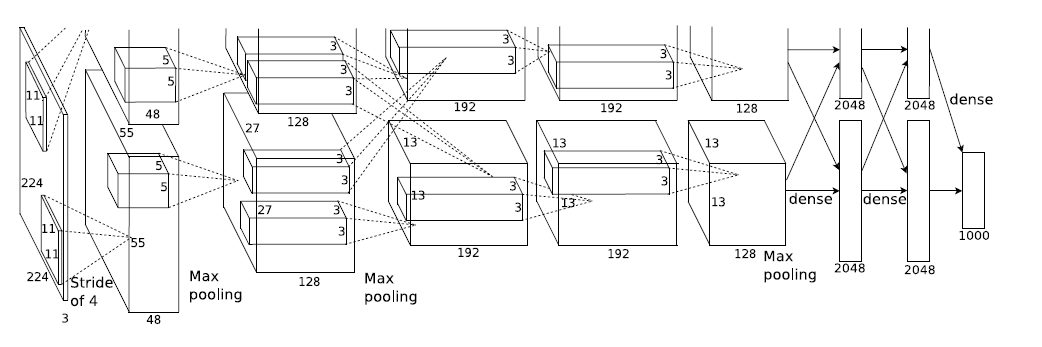
\includegraphics[width=0.8\textwidth]{figures/AlexNet-multiGPU.png}
	\caption{Topologia architektury AlexNet z podziałem na dwa akceleratory GPU.}
	\label{AlexNetTopologyMultiGPU}
\end{figure}

Topologia z podziałem na 2 karty zwiększyła dwukrotnie sumaryczną pamięć i pozwoliła na koalokację parametrów sieci.

Praca Alexa Krizhevsky, Ilya Sutskever i Geoffrey'a Hinton zapoczątkowała wzrost zainteresowania technikami głębokiego uczenia się, co doprowadziło do publikacji kolejnych podobnych architektur. Do najbardziej znanych należą ZFNet z 2013 roku [ZFNet], gdzie m.in. zastosowano zmniejszenie wymiaru jądra stosowanego w filtrach pierwszej warstwy konwolucyjnej do 7$\times$7 oraz VGGNet z 2014 roku, gdzie zastosowano większą liczbę warstw konwolucyjnych z mniejszym wymiarem jądra splotu. Innowacyjnym pomysłym, który został zaprezentowany również w 2014 było pojawienie się nowych modułów w sieci GoogleNet, która dokładniej została opisana w kolejnej podsekcji.

\subsection{GoogLeNet}

Architekturę o nazwie GoogLeNet zaprezentowano w 2014 r. w pracy [GoogleNet]. Nazwa architektury pochodzi od nazwy zwycięzkiego zespołu startującego w ILSVRC14, składającego się z pracowników firmy Google. Oryginalnie topologia składała się z 22 warstw i zawierała około 5 mln parametrów (12 razy mniej niż w przypadku sieci AlexNet). 

Redukcję liczby parametrów przy jednoczesnym podwyższeniu dokładności klasyfikacji i lokalizacji obiektów (zob. [ILSCV]) udało się uzyskać poprzez poszukiwania konstrukcji optymalnych lokalnych topologii i ich połączeń. Mianowicie, wiadomo że duża część funkcji aktywacji neuronów przyjmuje wartość 0 lub jest redundatna z powodu wysokiej korelacji między sobą (zob. [Arora z GoogleNet]). Matematyka dotycząca przetwarzania \textit{macierzy rzadkich}, tj. gdzie przeważająca liczba elementów przyjmuje wartość 0, jest dobrze znana np. [3-GoogleNet]. Jednak implementacje bibliotek do obliczeń związanych z algebrą liniową są zooptymalizowane pod kątem \textit{macierzy gęstych}, gdzie przeważająca liczba elementów przyjmuje wartości różne od 0 (zob. [16, 9 googleNet]). 

Ideą modułu incepcji zaproponowanego przez twórców GoogLeNet jest aproksymacja rzadkich macierzy z użyciem komponentów o gęstej strukturze. Takie komponenty nazwano \textit{modułami incepcji} (ang. \textit{inception modules}). Przykłądy modułów incepcji pokazano na Rys. \ref{GoogleNetInceptionModules} 
\begin{figure}[h!]
	\centering
	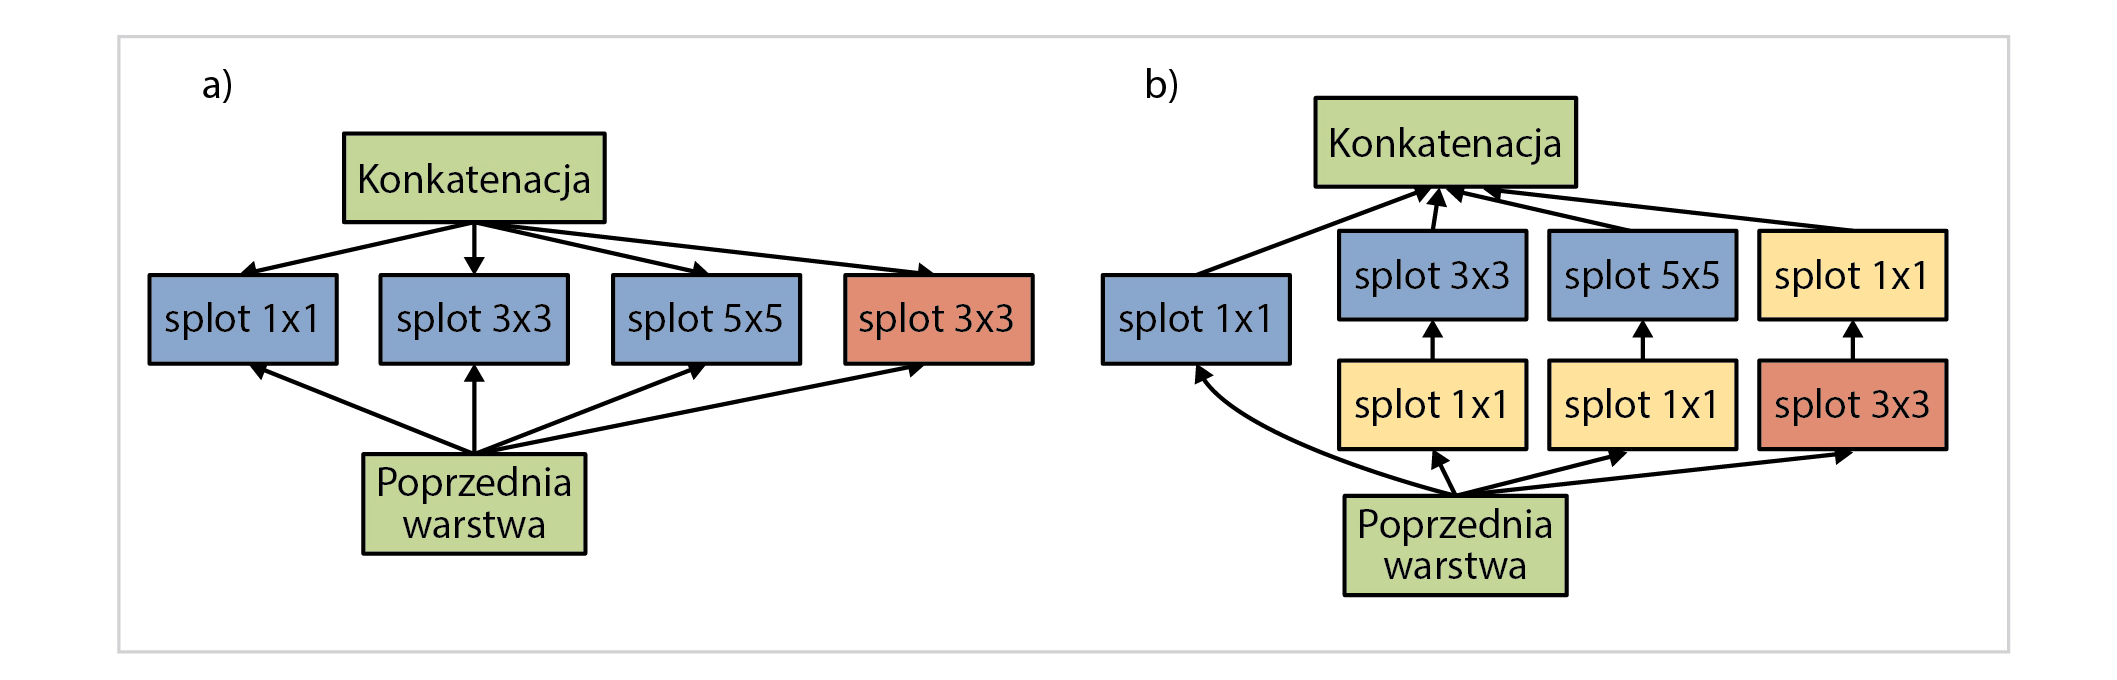
\includegraphics[width=0.8\textwidth]{figures/InceptionModules.png}
	\caption{Topologia architektury AlexNet z podziałem na dwa akceleratory GPU.}
	\label{GoogleNetInceptionModules}
\end{figure}

Rys. \ref{GoogleNetInceptionModules} (a) przedstawia najwną formę modułu incepcji, gdzie grupowane są operacje filtrów z jądrem o wymiarach 5$\times$5, 3$\times$3, 1$\times$1 oraz operacja max-pool. Rys. \ref{GoogleNetInceptionModules} (b) prezentuje koncepcję zooptymalizowaną obliczeniowo gdzie filtry 1$\times$1 służą do redukcji wymiarowości i używane są bezpośrednio przed splotami z bardziej wymagającymi obliczeniowo splotami z jądrami o wymiarach 5$\times$5 i 3$\times$3. 

Złożenie różnego rodzaju modułów dało topologię zaprezentowaną na Rys.
\begin{figure}[h!]
	\centering
	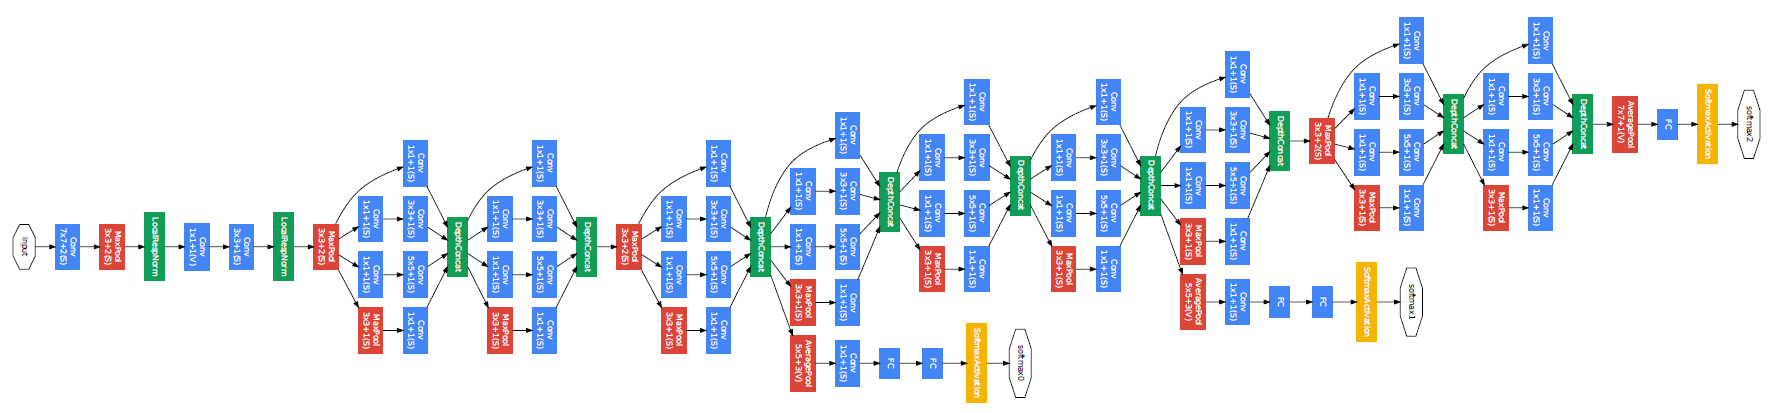
\includegraphics[width=1\textwidth]{figures/GoogleNet.png}
	\caption{Topologia architektury GoogleNet}
	\label{GoogleNetTopo}
\end{figure}

Dokładne zestawienie parametrów znajduje się w Tabeli \ref{GoogleNetParams}

\begin{table}[h!]
	\centering
	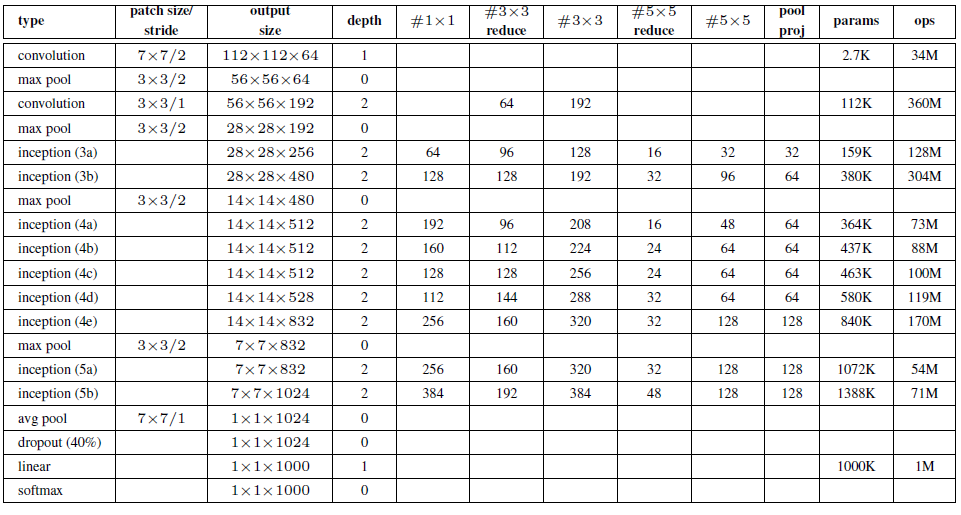
\includegraphics[width=1\textwidth]{figures/GoogleNetparams.png}
	\caption{Parametry architektury GoogleNet}
	\label{GoogleNetParams}
\end{table}

Ważną cechą sieci GoogleNet jest brak warstw typu FC na zakończeniu, gdzie w przypadku sieci AlexNet znajdowało się około 90\% parametrów. Końcowe wnioskowanie jest realizowane na podstawie wartości średniej z dwuwymiarowych map cech.

Dla lepszego zrozumienia idei redukcji wymiarowości realizowanej przez moduły incepcji, podobnie jak w przypadku sieci AlexNet, przeanalizowane zostanie działanie pierwszego modułu w topologii z Rys. \ref{GoogleNetTopo}.
Moduł zawiera 128 filtrów z jądrami o wymiarach 3$\times$3 i 32 filtry z jądrami o wymiarach 5$\times$5. Dane na wejściu modułu mają 192 kanały (zob. Tabela \ref{GoogleNetParams}). Dla przykładu, rząd wielkości obliczeń operacji splotów 32 filtrów 5$\times$5 wynosi 25$\times$32$\times$192=153 600 i dalej wzrastałby z głębokością sieci. W celu zapobiegnięcia nadmiarowi obliczeń stosowana jest redukcja z użyciem 16 filtrów z jądrem o wymiarach 1$\times$1. W efekcie rząd wielkości obliczeń spada do 16$\times$192 +  25$\times$32$\times$16=15 876, co pozwala na dalsze budowanie wielowarstwowych struktur.

Topologia GoogLeNet jest wciąż rozwijana. Po pierwszej prezentacji pojawiły się kolejne modernizacje wprowadzjące dodatkowe faktoryzacje modułów jak w Inception-v2 [Inception-v2], lub normalizacje wartości wynikowych poszczególnych warstw jak w Inception-v3 [Inception-v3]. Kolejny innowacyjny pomysł, bazujący na dodatkowych połączeniach między blokami, został wprowadzony w 2015 roku w sieci ResNet, która została opisana w kolejnej podsekcji.

\subsection{ResNet}

Jednym z najbardziej oczywistych pomysłów na polepszenie dokładności działania sieci neuronowych jest zwiększenie liczby warstw. Jednak wraz ze wzrostem liczby warstw, trening takich architektur z użyciem tradycyjnych metod gradientowych (takich jak algorytm wstecznej propagacji błędu) staje się mniej wydajny. Problem wynika z faktu, że zmiana wartości sygnału na wyjściu sieci w odpowiedzi na sygnał wejściowy jest mniejsza wraz ze wzrostem liczby warstw [ResNet]. W takiej sytuacji gradient wyliczany na podstawie sygnału będącego różnicą pomiędzy sygnałem wejściowym a wejściowym może przyjmować wartości bliskie 0 uniemożliwiając progres uczenia się. Problem zanikającego gradientu (ang. \textit{vanishing gradient problem}) rozwiązywany jest poprzez zastosowanie normalizacji oraz nieliniowych funkcji aktywacji, których przykłady zostały opisane w sekcji \ref{AlexNet} oraz szeroko w literaturze np. w [ResNet 2,3,4]. Dzięki tym mechanizmom algorytm treningu głębokich sieci neuronowych w większej liczbie przypadków zbiega do użytecznego minimum lokalnego. 

W momencie znalezienia takiego minimum dodanie kolejnych warstw i parametrów sieci jest redundatne, a nawet prowadzi do pogorszenia wyników treningu sieci, co związane jest z trudnościami optymalizacji przestrzeni wieloparametrycznych [Opt]. Zjawiskio to nosi nazwę degradacji treningu (ang. \textit{degradation problem}). Twórcy architektury ResNet zaproponowali rozwiązanie tego problemu poprzez implementację bloków rezydualnych (ang. \textit{Residuum Units}) zawierających dodatkowe, skrótowe połączenia (ang. \textit{skip conections}) pomiędzy wejściem a wyjściem bloków. Porównanie schematów funkcjonalnych nowych bloków i wcześniej istniejącego rozwiązania stosowanego np. w AlexNet został przedstawiony na Rys. \ref{ResNetBlock}.
\begin{figure}[h!]
	\centering
	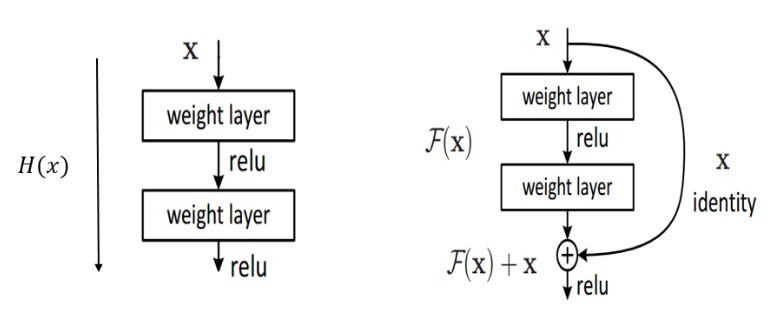
\includegraphics[width=0.5\textwidth]{figures/ResidualBlock.jpg}
	\caption{Schemat funkcjonalny pojedynczego bloku w architekturze ResNet.}
	\label{ResNetBlock}
\end{figure} 

Ogólną postać równania bloku rezydualnego można zapisać następująco:
\begin{equation}
\begin{split}
y_l = h(x_l) + F(x_l, W_l),\\
x_{l+1} = f(y_l),
\end{split}
\end{equation}
gdzie $x_l$ i $x_{l+1}$ stanowią sygnał wejściowy i wyjściowy $l$-tego bloku. $F$ stanowi funkcję rezydualną optymalizowaną podczas treningu sieci, $h$($x_l$) stanowi funkcję przekształcenia sygnału $x_l$ przekazywanego skrótowym połączeniem, $f$ jest funkcją ReLU, a $W$ stanowi macierz wag.

Funkcja $h$($x_l$) jest funkcją tożsamościową, a zatem $h$($x_l$) = $x_l$. Żeby uzasadnić ten wybór należy rozważyć propagację gradientu wewnątrz sieci skłądającej się z bloków rezydualnych. Dla każdego $L$-tego bloku zachodzi równanie:
\begin{equation}
x_L = x_l + \sum_{i=l}^{L-1}F(x_i, W_i)
\end{equation}
Korzystając z reguły łąńcuchowej [ResNet-wyj-9] można zapisać równanie na gradient funkcji kosztu $\varepsilon$:
\begin{equation}
\ref{gradResBlock}
\frac{\partial \varepsilon}{\partial x} =  \frac{\partial \varepsilon}{\partial x_L} \frac{\partial x_L}{\partial x_l} =  \frac{\partial \varepsilon}{\partial x_L}\left (1 +   \frac{\partial }{\partial x_l}\sum_{i=l}^{L-1}F(x_i, W_i) \right )
\end{equation}
z czego wynika, że gradient może być podzielony na dwie addytywne składowe: (1) $w$ = $\frac{\partial \varepsilon}{\partial x_L}$ propagowaną bez wpływu na warstwy zawierające wagi i (2) $\lambda$ = $\frac{\partial \varepsilon}{\partial x_L}\frac{\partial }{\partial x_l}\sum_{i=l}^{L-1}F(x_i, W_i)$ propagowaną przez nie.

Rozważając przykład sieci składający się z trzech bloków można zapisać:
\begin{equation}
\frac{\partial \varepsilon}{\partial x_0} =  \frac{\partial \varepsilon}{\partial x_3}*(w_2+\lambda_2)*(w_1+\lambda_1)*(w_0+\lambda_0)
\end{equation}

Można następnie wyszczególnić 4 przypadki:

(https://medium.com/@14prakash/understanding-and-implementing-architectures-of-resnet-and-resnext-for-state-of-the-art-image-cc5d0adf648e)
Przykład: lambda = gradient 
Case-1, Lambda = 0: This will be a plain network. Since w2, w1, w0 are all between {-1, 1}, the gradient vanishes as the network depth increases. This clearly shows vanishing gradient problem

Case-2, Lambda >1: In this case, The backprop value increases incrementally and lead to exploding of gradients.

Case-3, Lambda <1: For shallow networks this might not be problem. But for extra large networks, weight+lambda is still less than <1 in most cases and it achieves the same problem as case-1

case-4, Lambda =1: In this case, Every weight is incremented by 1, This eliminates the problem of multiplying with very large numbers as in case-2 and small numbers as in case-1 and acts as a good barrier.

Kompletna sieć zaproponowana w 2015 roku została pokazana na Rys.:
(wstaw rysunek topo)


 Warianty ResNet: (https://towardsdatascience.com/an-overview-of-resnet-and-its-variants-5281e2f56035)

\subsection{Złożenia}
\section{Zastosowania w medycynie}
